\documentclass[
	12pt,
	oneside,
	a4paper,
	english,
	brazil
]{abntex2ppgsi}

\usepackage[utf8]{inputenc} 
\usepackage{lastpage}
\usepackage{indentfirst}
\usepackage{color}
\usepackage{graphicx}
\usepackage{microtype}
\usepackage{pdfpages}
\usepackage{algorithm}
\usepackage{mdwlist}
\usepackage[noend]{algpseudocode}

\usepackage{hyperref}
\usepackage[brazilian,hyperpageref]{backref}
\usepackage[alf,abnt-etal-list=0,abnt-etal-text=it]{abntex2cite}

\renewcommand{\backrefpagesname}{Citado na(s) página(s):~}
\renewcommand{\backref}{}
\renewcommand*{\backrefalt}[4]{
	\ifcase #1 
		Nenhuma citação no texto.
	\or
		Citado na página #2.
	\else
		Citado #1 vezes nas páginas #2.
	\fi}

\instituicao{
	UNIVERSIDADE DE SÃO PAULO
	\par
	ESCOLA DE ARTES, CIÊNCIAS E HUMANIDADES
	\par
	CURSO DE BACHARELADO EM SISTEMAS DE INFORMAÇÃO}

\titulo{Os efeitos do agendamento midiático nas redes sociais: um estudo de caso no contexto das eleições de 2022 no Brasil}

\autor{\uppercase{Igor Antun da Costa Gago}}
\local{São Paulo}
\data{2023}
\orientador{Prof. Dr. Marcio Moretto Ribeiro}
\tipotrabalho{Monografia de Conclusão de Curso}

\preambulo{
\newline \newline \newline 
Monografia apresentada à Escola de Artes, Ciências e Humanidades da Universidade de São Paulo, como parte dos requisitos exigidos na disciplina ACH 2018 - Projeto Supervisionado ou de Graduação II, para obtenção do título de Bacharelado em Sistemas de Informação.
\newline \newline Modalidade: TCC longo (1 ano) - individual
\newline }

\definecolor{blue}{RGB}{41,5,195}

\makeatletter
\hypersetup{
		pdftitle={\@title}, 
		pdfauthor={\@author},
    	pdfsubject={\imprimirpreambulo},
	    pdfcreator={laTeX com abnTeX2 adaptado para o PPgSI-EACH-USP},
		pdfkeywords={abnt}{latex}{abntex}{abntex2ppgsi}{monografia}{bsi}, 
		colorlinks=true,
    	linkcolor=blue,
    	citecolor=blue,
    	filecolor=magenta,
		urlcolor=blue,
		bookmarksdepth=4
}
\makeatother

\setlength{\parindent}{1.25cm}
\setlength{\parskip}{0cm} 
\renewcommand{\baselinestretch}{1.5}

\makeindex

\clubpenalty10000
\widowpenalty10000
\displaywidowpenalty10000

\begin{document}

\frenchspacing 

\pretextual

\imprimircapa

\imprimirfolhaderosto*

% ---
% Dedicatória
% ---
%-------------------------------------------------------------------------
% Comentário adicional do PPgSI - Informações sobre ``Dedicatória'': 
%
% Opcional 
% 
%-------------------------------------------------------------------------
%\begin{dedicatoria}
%   \vspace*{\fill}
%   \centering
%   \noindent
%   \textit{Escreva aqui sua dedicatória, se desejar, ou remova esta página...}
%\vspace*{\fill}
%\end{dedicatoria}
% ---
%
% ---
% Agradecimentos
% ---
%-------------------------------------------------------------------------
% Comentário adicional do PPgSI - Informações sobre ``Agradecimentos'': 
%
% Opcional 
% 
% Financiamentos recebidos durante o projeto, vindos de qualquer 
% agência de fomento, devem ser mencionados na seção de agradecimentos da monografia. 
% Isso se aplica não apenas a bolsas de estudo, mas a qualquer tipo de financiamento, 
% tais como para apoio a participação em eventos, compra de materiais, traduções etc. 
%
%
%-------------------------------------------------------------------------
%\begin{agradecimentos}
%\end{agradecimentos}
% ---

% ---
% Epígrafe
% ---
%-------------------------------------------------------------------------
% Comentário adicional do PPgSI - Informações sobre ``Epígrafe'': 
%
% Opcional para Dissertação/Tese.
% Não sugerido para Qualificação.
% 
%-------------------------------------------------------------------------
%\begin{epigrafe}
%    \vspace*{\fill}
%	\begin{flushright}
%		\textit{``Escreva aqui uma epígrafe, se desejar, ou remova esta página...''\\
%		(Autor da epígrafe)}
%	\end{flushright}
%\end{epigrafe}

% ---

\setlength{\absparsep}{18pt}
\begin{resumo}

\begin{flushleft}
GAGO, Igor Antun da Costa. \textbf{Os efeitos do agendamento midiático nas redes sociais}: um estudo de caso no contexto das eleições de 2022 no Brasil. \imprimirdata. \pageref{LastPage} f. Monografia (Bacharelado em Sistemas de Informação) – Escola de Artes, Ciências e Humanidades, Universidade de São Paulo, São Paulo, 2022.
\end{flushleft}

A hipótese do agendamento propõe que grandes veículos midiáticos, apesar de não influenciarem diretamente \textit{o que} as pessoas pensam sobre determinadas questões, possuem o grande poder de determinar \textit{quais} serão as questões de destaque na sociedade em um dado momento. No entanto, com a adoção em massa das mídias sociais, o público é exposto a uma variedade maior de fontes de notícia e possui influência direta na relevância que é dada a uma matéria. O presente estudo buscou entender, através da aplicação de técnicas automatizadas de raspagem de dados, a correlação entre a importância dada pelos jornais à uma notícia e a que lhe é dada nas redes sociais (Facebook e Twitter), no contexto das eleições presidenciais de 2022 no Brasil. Dentre os 10 cenários analisados, apenas 1 apontou para uma possível correlação entre estas. Isto é, dentro dos dados obtidos, verificou-se que na maior parte dos casos tal correlação é inexistente. 

Palavras-chaves: Teoria do agendamento; Mídia; Redes sociais; Agenda pública; Eleições;
\end{resumo}

\begin{resumo}[Abstract]
\begin{otherlanguage*}{english}

\begin{flushleft}
GAGO, Igor Antun da Costa. \textbf{The effects of media agenda-setting on social networks}: A case study in the context of 2022 Brazilian general elections. \imprimirdata. \pageref{LastPage} p. Monograph (Bachelor of Information Systems) – School of Arts, Sciences and Humanities, University of São Paulo, São Paulo, 2022. 
\end{flushleft}

The agenda-setting theory suggests that media institutions — despite being unable to directly influence \textit{what} people think about a set of issues — have the great power of determining \textit{which} issues are most important to society in a given moment. With the mass adoption of social networks, though, the public is exposed to a greater amount of news sources and have direct influence in the relevance given to a topic. The present study aimed to understand, through the use of automatic data scraping techniques, the correlation between the relevance given by newspapers to an article and the one given to it in the social networks (Facebook and Twitter), in the context of 2022 Brazilian general elections. Out of 10 analyzed scenarios, only 1 pointed towards a possible correlation between those. That is, given the obtained data, it was concluded that said correlation is inexistent in the vast majority of scenarios.

Keywords: Agenda-setting; Media; Social networks; Public agenda; Elections;
\end{otherlanguage*}
\end{resumo}

\pdfbookmark[0]{\listfigurename}{lof}
\listoffigures*
\cleardoublepage

\pdfbookmark[0]{\listtablename}{lot}
\listoftables*
\cleardoublepage

\begin{siglas}
  \item[API] Interface de programação de aplicações, em inglês
\end{siglas}

\begin{simbolos}
  \item[$ \rho $] Coeficiente de correlação de Spearman
\end{simbolos}

\pdfbookmark[0]{\contentsname}{toc}
\tableofcontents*
\cleardoublepage

\textual

\chapter{Introdução}
A hipótese do agendamento (\textit{agenda-setting}) propõe que grandes veículos midiáticos, apesar de não influenciarem diretamente \textit{o que} as pessoas pensam sobre determinadas questões, possuem o grande poder de determinar \textit{quais} serão as questões de destaque na sociedade em um determinado momento, em detrimento de outras \cite{mccombs}.

Historicamente o consumo de notícias se deu majoritariamente de forma passiva, através de meios como o jornal impresso, o rádio ou a televisão \cite{ahlers}. Nesse contexto, as escolhas feitas pela equipe editorial de um jornal possuem efeitos diretos na disseminação de informação e percepção de relevância de uma pauta. Com a adoção em massa das mídias sociais, no entanto, o público geral é exposto a uma variedade crescente de fontes de notícias \cite{sterrett}. Sejam essas legítimas ou falsas, de jornais tradicionais ou de páginas pessoais, todas competem pelos mesmos espaços de destaque.

A decisão editorial, agora decentralizada, é diretamente influenciada pelo engajamento dado por usuários nas redes sociais e pelos algoritmos que as regem. Os atores envolvidos no debate e difusão de uma notícia muitas vezes são mais relevantes que o próprio conteúdo da notícia compartilhada \cite{chen}, e têm um grande papel em determinar o alcance de uma notícia.

A relevância que de outra forma seria atribuída pela decisão de poucas pessoas, agora é portanto produto das interações entre inúmeras pessoas e fatores. Essa configuração pode gerar um descasamento entre o que é destacado pela mídia e o que é priorizado no debate público, como previamente observado nas eleições brasileiras de 2010 por \citeonline{nunomura}.

As consequências da influência das redes sociais no debate político puderam ser observadas em maior intensidade no ano de 2016, durante as eleições presidenciais nos Estados Unidos \cite{allcott}. Marcada por intensas campanhas de disseminação de notícias falsas, mostrou de forma prática que, com a decentralização das formas de obtenção e distribuição de notícias, a fonte não é mais tão importante ao ler ou compartilhar algo. Segundo \citeonline{gottfried}, 62\% dos adultos americanos obtém notícias através de redes sociais, onde circulam com facilidade e sem muitos filtros ou checagem de fatos. Durante o período eleitoral, notícias falsas representaram aproximadamente 6\% das notícias consumidas no Twitter \cite{grindberg}.

Este trabalho busca entender, através de um estudo longitudinal e da aplicação de técnicas automatizadas de raspagem de dados, a correlação entre a importância dada pela agenda midiática a uma matéria jornalística em jornais digitais e a que lhe é atribuída pela agenda pública nas redes sociais, no contexto das eleições presidenciais de 2022 no Brasil.

\section{Conceitos e definições}
Ao longo do texto são utilizados termos e conceitos específicos ao contexto do presente trabalho. Estes estão definidos da seguinte forma:
\begin{itemize}
    \item \textbf{Agendamento midiático:} Processo pelo qual as plataformas midiáticas selecionam os fatos a serem noticiados e questões a serem discutidas, em detrimento de outras. É em grande parte responsável, portanto, pelo que o público geral sabe e se importa em um dado momento. Nesse sentido, a agenda midiática é o conjunto de questões selecionadas pela mídia para terem importância naquele momento.
    \item \textbf{Agenda pública:} A agenda pública, por sua vez, é definida pelo conjunto de questões e fatos escolhidos pela população para receber atenção em um dado momento. Com a popularização das redes sociais, qualquer pessoa é capaz de contribuir para sua construção, promovendo engajamento às notícias que julgar serem mais relevantes.
    \item \textbf{Raspagem de dados:} Técnica de mineração de dados, pela qual um programa extrai dados acessíveis em sites e plataformas digitais e os converte em informação estruturada para análise futura.
    \item \textbf{Saliência:} Grau de relevância ou proeminência dado a uma matéria jornalística específica, por um determinado agente. No contexto de um jornal, deriva do destaque dado por sua equipe editorial em termos de tempo de exposição e posição hierárquica entre as demais matérias. Já nas redes sociais, deriva do engajamento dado pelas pessoas a uma matéria. Será utilizada para metrificar e comparar quantitativamente a atenção recebida pelas matérias jornalísticas observadas.
    \item \textbf{Script:} Programa de computador automatizado para execução de um determinado conjunto de instruções.
\end{itemize}

\section{Justificativa}
Ao ditar quais serão as questões de maior relevância para o debate público, um agente efetivamente limita as opções de temas que serão tratados na sociedade e em suas políticas públicas \cite{mccombs}. Estudar o impacto do agendamento nas plataformas digitais sociais e midiáticas, portanto, é uma importante ferramenta para entendermos sua influência no contexto da mudança social.

Com o crescente aumento do uso de redes sociais e de \textit{fake news} com intuito político, cresce também a preocupação acerca de tentativas de manipulação da opinião pública \cite{zhuravskaya}. Desde 2010, partidos políticos e governos investiram mais de meio bilhão de dólares na pesquisa, desenvolvimento e implementação de operações psicológicas e manipulação da opinião pública através de redes sociais \cite{bradshaw}. Especificamente entre os países em desenvolvimento, há forte evidência da operação de tais campanhas em plataformas de conversação como WhatsApp, WeChat e Telegram.

Dado o cenário de intensa tentativa de manipulação do debate político, surge o interesse em analisar até que ponto o conteúdo compartilhado nas redes sociais acompanha as matérias jornalísticas dadas como mais relevantes pela mídia. 

Há, portanto, a oportunidade de reavaliar estudos como o de \citeonline{nunomura} e \citeonline{allcott} com um novo olhar, trazendo-os para o período eleitoral do Brasil de 2022, visando traçar conexões entre o que é priorizado no espaço editorial jornalístico e o que é priorizado pelo público geral no debate virtual.


\section{Proposição}
O presente estudo de caso possui a intenção de analisar os efeitos do agendamento midiático no contexto das eleições presidenciais no Brasil em 2022. Através da observação conjunta e sistemática do destaque dado a uma publicação nos cinco principais portais jornalísticos do país (\textit{Estadão}, \textit{Folha de S. Paulo}, \textit{g1}, \textit{UOL} e \textit{Veja}) e o engajamento obtido por estas nas redes sociais Facebook e Twitter, pretende-se mensurar e analisar a eventual correlação entre suas agendas.

Ainda que uma correlação não implique relação de causalidade, seu resultado pode dar pistas de como as agendas públicas e midiáticas interagem entre si. Trabalhos futuros podem explorar a análise dos resultados aqui obtidos em conjunto com novos dados e observações, de modo a identificar outros fatores que potencialmente influenciem a relação entre essas.

Importante também ressaltar que o presente trabalho se restringe à comparação da saliência conferida por uma mesma matéria jornalística nas diferentes plataformas observadas (jornais digitais, Facebook e Twitter). Isto significa acompanhar nestas as métricas ao redor do \textit{link} da matéria. O estudo não se propõe a realizar análise e acompanhamento de assuntos ou tópicos, e portanto desconsidera publicações que não contenham o \textit{link} de uma notícia.


\section{Objetivos}
\subsection{Objetivo geral}
Mensurar e analisar a correlação entre a saliência atribuída à uma matéria em portais jornalísticos (agenda midiática) e o engajamento obtido por ela nas redes sociais Facebook e Twitter (agenda pública).

\subsection{Objetivos específicos}
\begin{itemize}
    \item Desenvolver uma aplicação para execução automatizada da raspagem de dados e notícias de \textit{sites} de jornais. Disponibilizar publicamente seu código-fonte para que possa ser utilizada em outros contextos.
\end{itemize}


\section{Método}
O presente trabalho trata de uma pesquisa aplicada e exploratória, realizada através de estudo de caso empírico. Seus cálculos e conclusões foram alcançados através da observação direta e da análise quantitativa de indicadores de saliência de matérias jornalísticas em jornais digitais e redes sociais durante o período eleitoral brasileiro de 2022, na intenção de estudar a correlação entre as agendas dessas plataformas.

A fim de comparar a saliência dada a uma determinada matéria nos portais jornalísticos e nas redes sociais, é necessário primeiro obter os dados brutos necessários e tratá-los de forma a possibilitar a análise. Cada meio aqui analisado necessitou de uma forma distinta de obtenção de dados.

Para o monitoramento dos portais jornalísticos, foi desenvolvido um \textit{script} automatizado que aplica técnicas de raspagem de dados objetivando a guardar o histórico das matérias publicadas na página inicial dos jornais analisados.

Na rede social Twitter foi utilizada sua API de busca histórica, a fim de encontrar publicações com referência direta ao \textit{link} das matérias identificadas pelo \textit{script} anterior e armazenar métricas acerca de seu engajamento. As métricas do Facebook, por sua vez, foram obtidas com o uso da ferramenta CrowdTangle, que oferece acesso ao arquivo histórico de publicações do Facebook e também a seus dados atualizados.

Por fim, com todas os dados necessários obtidos dos portais jornalísticos, do Facebook e do Twitter, foi realizada a análise de correlação das métricas de saliência. Para isso, foi escrito um \textit{script} na linguagem R.


\section{Limitações}
\begin{itemize}
    \item Para mensurar o engajamento obtido por uma matéria jornalística nas redes sociais, foi realizada uma busca em cada rede (Facebook e Twitter) com base no \textit{link} da matéria no portal. Ou seja, o cálculo de engajamento se restringe às publicações que continham em seu conteúdo o endereço específico da matéria em questão. Por consequência, diversos tipos de publicação potencialmente referentes à mesma matéria (porém não contendo seu \textit{link} original) não foram considerados no estudo, como:
    \begin{itemize}
        \item Publicações contendo apenas trechos textuais da matéria;
        \item Publicações compartilhadas em forma de imagem;
        \item Publicações contendo versões alternativas ou reduzidas do \textit{link} da matéria original.
    \end{itemize}
    \item A observação automatizada dos portais jornalísticos compreendeu o período de 16 de outubro à 13 de novembro de 2022. Foram observadas as duas semanas anteriores e posteriores ao segundo turno do período eleitoral.
    \item Os dados de engajamento foram obtidos e calculados após a janela de observação dos jornais, de forma pontual. Isto é, foram coletados os números totais e acumulados de interações durante todo o período, uma única vez, sem dimensão temporal.
\end{itemize}

\chapter{Método}

\section{Raspagem de dados dos jornais}

O \textit{script} desenvolvido foi configurado de forma a ser executado em intervalos regulares de 1 hora (podendo ter o intervalo facilmente alterado). A cada execução, são acessados os cinco principais portais jornalísticos do país: \textit{Estadão}, \textit{Folha de S. Paulo}, \textit{g1}, \textit{UOL} e \textit{Veja}. Uma vez acessada a página inicial do jornal, são coletados dados acerca das 5 principais publicações.

Ao fim de cada execução, são exportados relatórios em 4 formatos diferentes:
\begin{itemize}
    \item \textit{.json}: Relatório principal, contendo o resultado do processamento da raspagem de dados. Inclui, para cada publicação encontrada, seu \textit{link}, título, descrição, chapéu (uma ou duas palavras usadas para definir o assunto da matéria, geralmente acima da manchete), espaço ocupado na tela em \textit{pixels}, coordenadas na tela e posição hierárquica entre as demais matérias.
    \item \textit{.html}: Página original na íntegra, acessível localmente com imagens, \textit{links}, menus e botões em sua maioria funcionais. Especialmente importante como forma de \textit{backup}, uma vez que caso alguma falha ocorra na raspagem de dados é possível revisitar o conteúdo original da página e analisá-lo novamente. Sem isso, uma falha no \textit{script} de raspagem poderia ocasionar perda de dados importantes, dada a constante rotatividade de conteúdo dos jornais.
    \item \textit{.pdf}: Página exportada em formato de documento, com imagens, texto selecionável, rolagem de conteúdo e \textit{links} funcionais.
    \item \textit{.webp}: Captura de tela da página no momento de acesso, limitada ao tamanho da janela de exibição configurada
\end{itemize}

Finalmente, uma vez gerados os relatórios, os mesmos são armazenados para posterior análise.

\section{Raspagem de dados das redes sociais}
Para obter as métricas de engajamento das matérias jornalísticas dentro das redes sociais, técnicas diferentes precisaram ser empregadas. Em cada caso foi necessário levar em consideração as limitações das APIs disponíveis e a diferença entre os dados disponibilizados.

\subsection{Extração de dados do Twitter}

Na rede social Twitter foi utilizada sua API pública, que permite a busca de publicações específicas e a quantidade de interações obtidas por estas. Seu método de busca foi utilizado para encontrar todas as publicações (\textit{tweets}) contendo referência direta ao \textit{link} das matérias identificadas pelo \textit{script} supracitado. As métricas de engajamento, como ``curtidas", respostas e republicações (\textit{retweets}) são, por fim, armazenados.

Para cada notícia buscada, os seguintes dados foram extraídos:
\begin{itemize}
    \item \textit{resultCount}: Total de publicações encontradas na busca
    \item \textit{likeCount}: Total de "curtidas"
    \item \textit{retweetCount}: Total de compartilhamentos
    \item \textit{replyCount}: Total de comentários
    \item \textit{quoteCount}: Total de citações
\end{itemize}

\subsection{Extração de dados do Facebook}

Os dados do Facebook, por sua vez, foram obtidos com o uso da API da plataforma CrowdTangle, que oferece acesso ao arquivo histórico de publicações do Facebook e também a seus dados atualizados. Através da mesma, também é possível buscar publicações que contenham um \textit{link} específico, e, assim como com o Twitter, armazenar suas métricas de engajamento: reações (curtidas e outras), comentários e compartilhamentos.

Para cada notícia buscada, os seguintes dados foram extraídos:
\begin{itemize}
    \item \textit{likeCount}: Total de "curtidas"
    \item \textit{shareCount}: Total de compartilhamentos
    \item \textit{commentCount}: Total de comentários
    \item \textit{loveCount}, \textit{careCount}, \textit{wowCount}, \textit{hahaCount}, \textit{sadCount} e \textit{angryCount}: Total das demais reações disponíveis
\end{itemize}

\section{Tratamento e análise dos dados}
Ao final do período de obtenção de dados foram geradas duas bases separadas de dados: uma para a rede social Facebook, e outra para o Twitter. Cada uma dessas listas contendo: endereço da matéria, portal jornalístico, saliência mensurada no portal, saliência mensurada na rede social.

\subsection{Tratamento dos dados}
Em ambas as redes sociais, observou-se um número significativo de casos em que publicações contendo o \textit{link} da matéria não foram encontradas, ou em que não houve nenhum engajamento. Para que uma análise mais clara pudesse ser feita, optou-se por remover das bases de dados as matérias cuja saliência mensurada nas redes sociais fosse nula.

\subsection{Análise dos dados}
Em razão das especificidades das diferentes redes sociais e jornais analisados, os dados obtidos apresentaram grandes variações em magnitude. Isto é, o valor absoluto da saliência calculada para uma dada matéria varia significativamente a depender do jornal ou rede social em questão.

Dado isso, optou-se por utilizar o método de Spearman para identificar eventuais correlações entre as aparições de uma notícia nos portais jornalísticos e o engajamento obtido pela mesma nas redes sociais. A correlação de Spearman utiliza a posição ordenada dos itens (\textit{ranking}), ao invés de seus valores absolutos. Dessa forma foi possível focar na proporcionalidade das saliências, e não na relação exata entre seus valores numéricos.


\chapter{Resultados}
Nessa seção exploraremos os dados gerados pela pesquisa e entraremos nos detalhes dos resultados obtidos com suas análises. 
Em todos os casos, empregou-se a mesma fórmula de correlação e portanto os mesmos critérios de interpretação. Para o método de Spearman, isso significa:
\begin{itemize}
    \item Analisar o coeficiente de correlação ($\rho$). Um valor 0 aponta inexistência de correlação, enquanto -1 ou +1 equivalem à uma correlação perfeita negativa ou positiva.
    \item Considerar a probabilidade de significância (p-valor). Este varia entre 0 e 1 e indica a probabilidade da correlação observada se dar ao acaso. Um valor próximo a 1 sugere que não há correlação fora o acaso, e portanto valida a hipótese nula. Um valor próximo a 0 (nesse caso, abaixo de 0,05), no entanto, rejeita a hipótese nula e reforça a evidência obtida pelo coeficiente de correlação.
\end{itemize}

Coeficientes de correlação individuais foram calculados para cada jornal analisado, dentro de cada rede social. Dessa forma foi possível isolá-los e compreender também suas diferenças quanto ao uso das plataformas sociais e o engajamento que possuem em cada. Estes estão apresentados abaixo em forma de gráficos independentes, e também em tabelas equivalentes.

Nos gráficos, cada ponto representa uma matéria jornalística. O eixo horizontal representa a saliência conferida a ela no portal jornalístico, considerando seu tempo e hierarquia de exibição. O eixo vertical, por sua vez, indica o número total de interações acumuladas na rede social em questão por publicações que contenham o endereço da mesma matéria. Há também, em cada gráfico, a regressão linear advinda de sua correlação, junto a seu intervalo de confiança.

Como poderá ser observado a seguir, os dados não apresentam tendência clara e em muitos casos estão espalhados de forma aparentemente desordenada. Isso pode, em certa medida, ser atribuído a algumas limitações do estudo como a janela de tempo observada e dificuldades na busca de publicações. No entanto, é possível que haja relação também com a forma como os jornais utilizam as redes sociais e a presença que têm nas mesmas: frequência de publicação, número de seguidores, etc.

\section{Resumo dos dados obtidos}
Através da raspagem de dados, foi possível obter o seguinte quantitativo de matérias:

\begin{table}[H]
	\centering
	\caption{Total de notícias observadas por jornal}
		\begin{tabular}{p{2in} p{1in} p{1in} p{1in} } \hline

		Jornal & Notícias \\ \hline
		Estadão	& 706 \\ 
		Folha de S.Paulo & 543 \\ 
		g1	& 787 \\ 
		UOL	& 747 \\
		Veja & 336 \\ \hline
        Total & 3119 \\ \hline
		
		\end{tabular}
	\label{tab:total-noticias}
  \source{Igor Antun, 2023}
\end{table}

Entretanto, para evitar disparidades na análise, subtraímos do conjunto de dados as matérias cujos \textit{links} não tivessem sido compartilhados em ambas as redes sociais (tanto Facebook quanto Twitter). Após a desconsideração dos 53 casos encontrados, restaram 3066 matérias a serem analisadas.

\section{Facebook}

\begin{table}[H]
	\centering
	\caption{Engajamento observado no Facebook}
		\begin{tabular}{p{2in} p{1in} p{1in} p{1in} } \hline

		Ação              & Média & Máximo \\ \hline
		Curtidas	      & 473   & 44248 \\ 
		Compartilhamentos & 70    & 7216 \\ 
		Comentários       & 306   & 18611 \\ \hline
		
		\end{tabular}
	\label{tab:engajamento-facebook}
  \source{Igor Antun, 2023}
\end{table}

\begin{figure}[H]
	\centering
 	  \caption{Correlação entre saliência nos jornais online e interações no Facebook}
		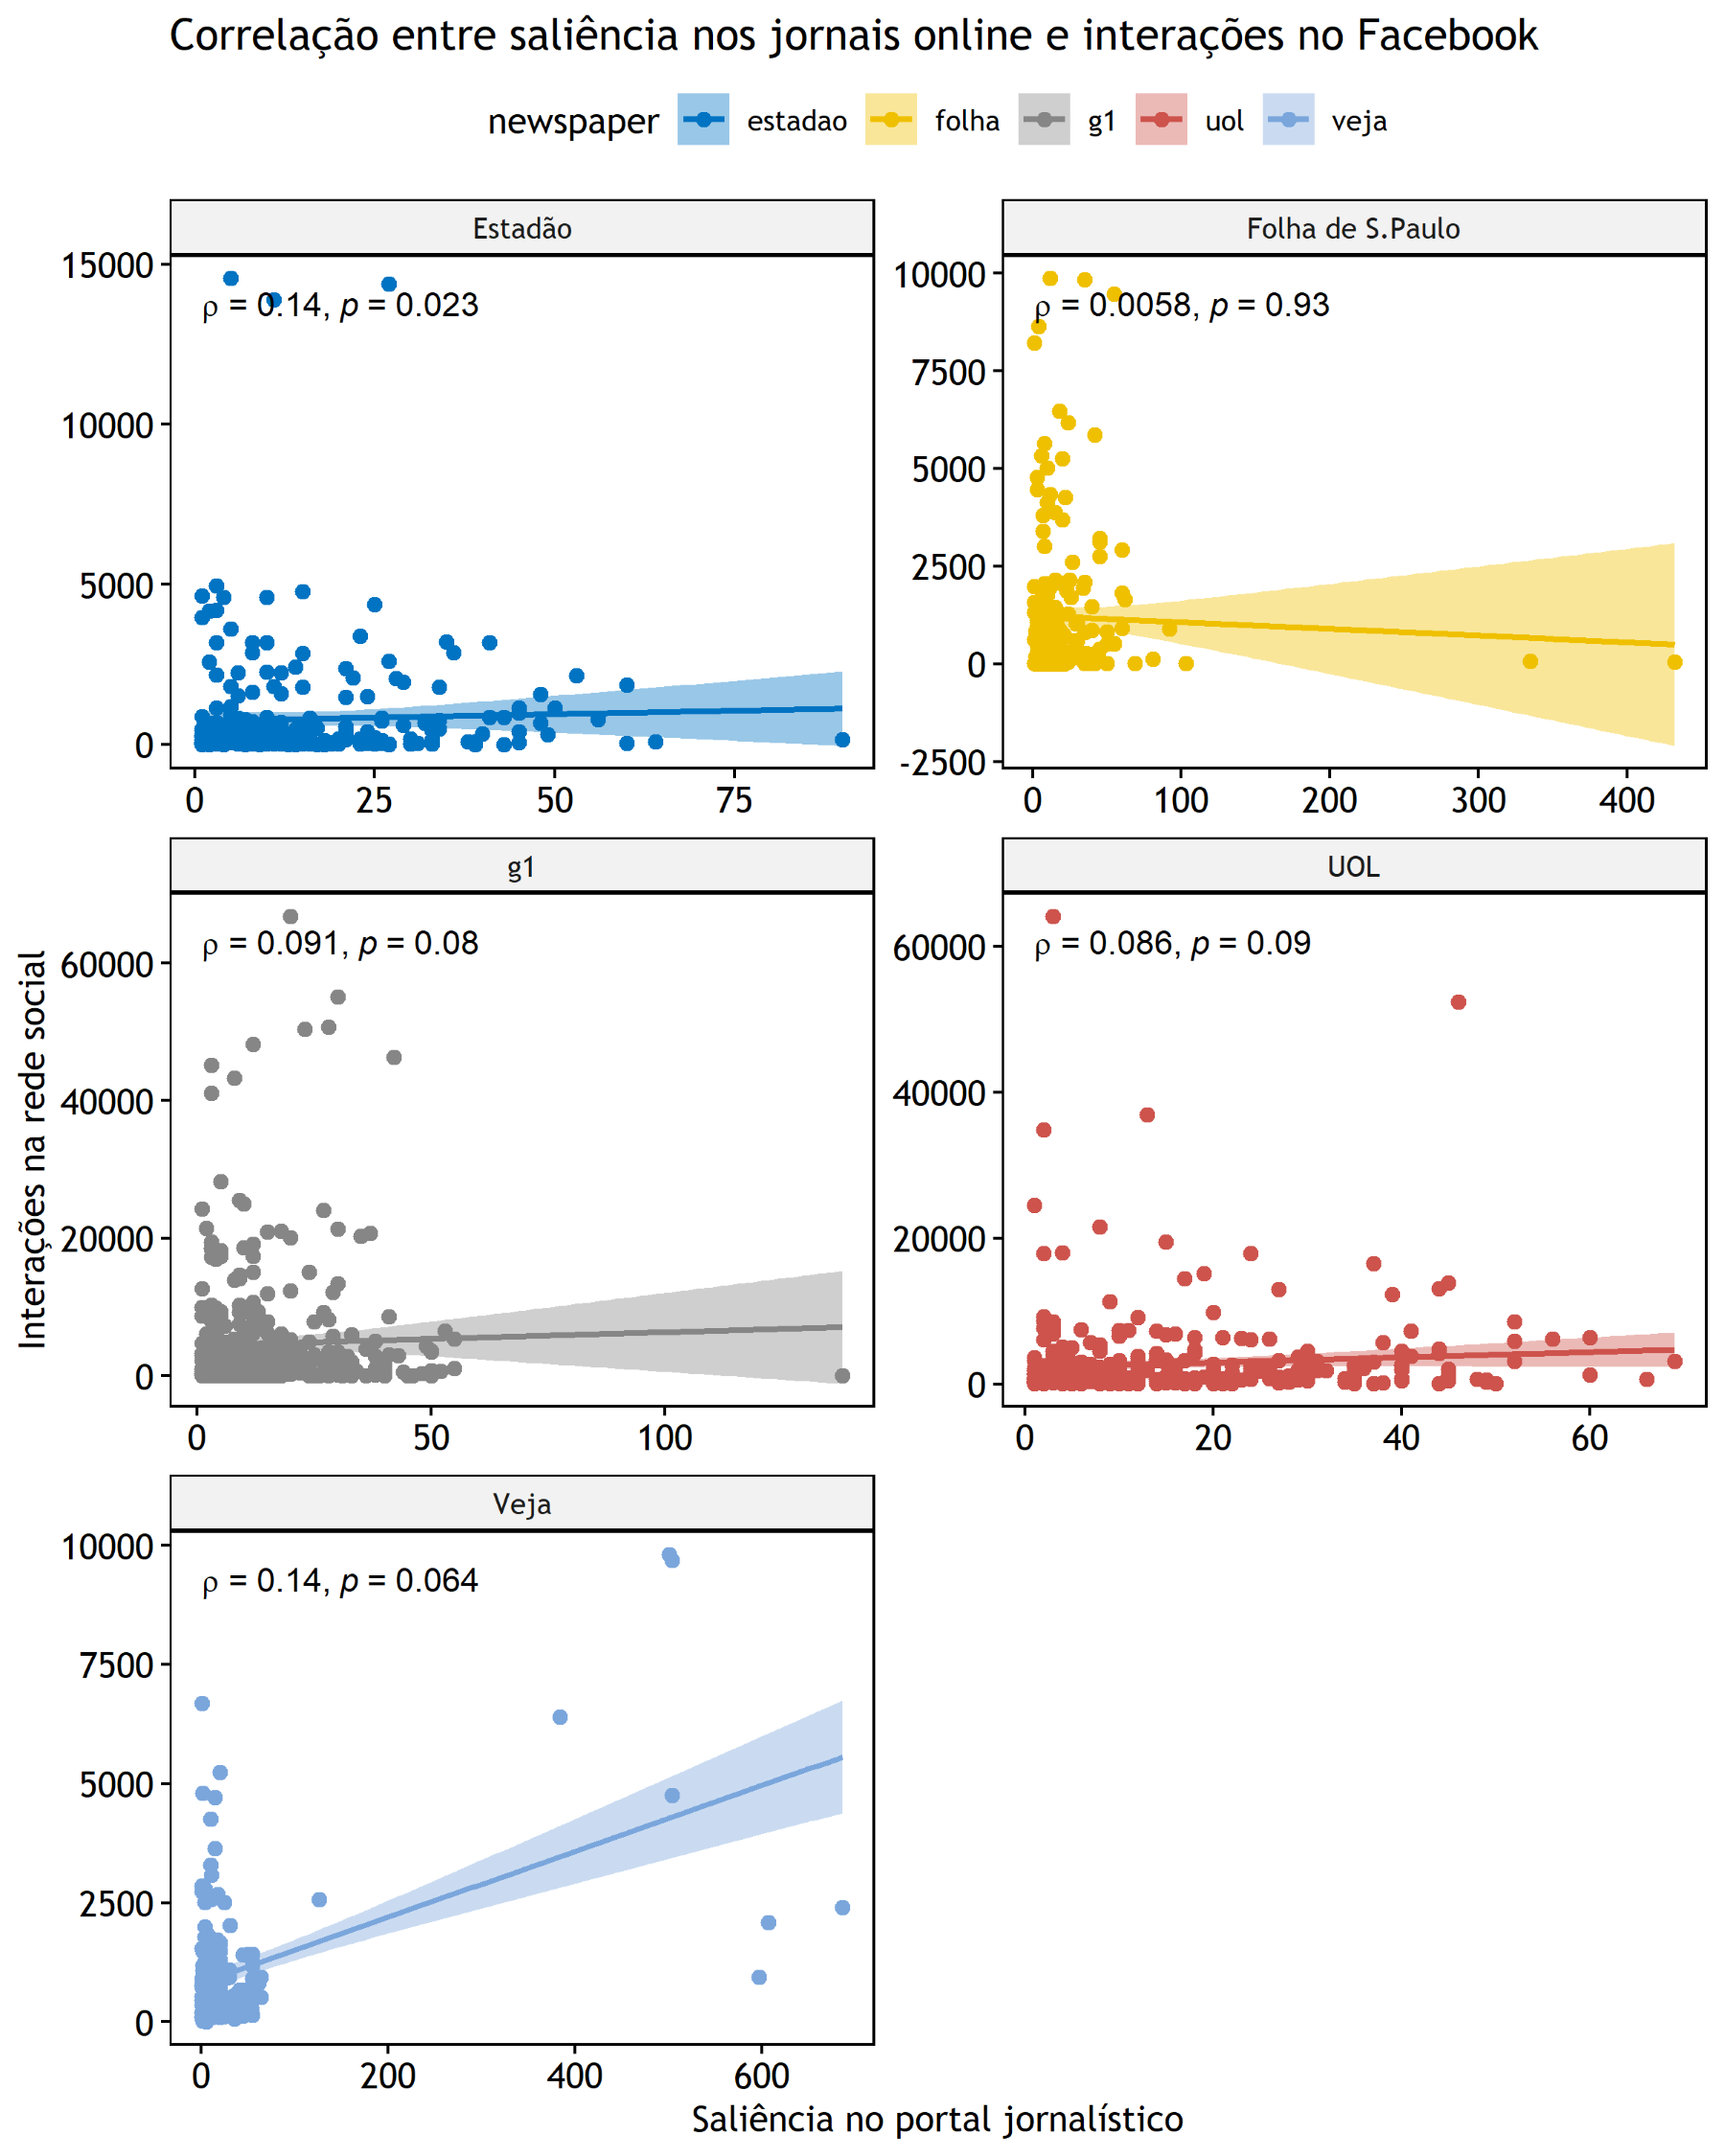
\includegraphics{facebook.png}
	\label{fig:correlacao-facebook}
  \source{Igor Antun, 2023}
\end{figure}

\begin{table}[H]
	\centering
	\caption{Correlação de Spearman - Facebook}
		\begin{tabular}{p{2in} p{1in} p{1in} p{1in} } \hline

		Jornal & $\rho$ & p-valor \\ \hline
		Estadão	& 0,14 & 0,023 \\ 
		Folha de S.Paulo & 0,0058 & 0,93 \\ 
		g1	& 0,091 & 0,08 \\ 
		UOL	& 0,086 & 0,09 \\ 
		Veja & 0,14 & 0,064 \\ \hline
		
		\end{tabular}
	\label{tab:correlacao-facebook}
  \source{Igor Antun, 2023}
\end{table}

Aqui podemos observar que somente o Estadão e a Veja obtiveram coeficientes de correlação acima de 0,1, o que no entanto ainda evidencia a inexistência de uma correlação. Em todos os outros casos, os valores foram ainda menores.

É importante notar também que, para quase todos os jornais, o p-valor obtido também estava acima do limiar aceitável de 0,05 (ou 5\%), novamente tendo o Estadão como exceção.

Considerando os coeficientes de correlação quase nulos e também os p-valores altos, os dados apontam para a ausência de qualquer correlação entre os eixos.

\section{Twitter}

\begin{table}[H]
	\centering
	\caption{Engajamento observado no Twitter}
		\begin{tabular}{p{2in} p{1in} p{1in} p{1in} } \hline

		Ação              & Média & Máximo \\ \hline
		Curtidas	      & 1161  & 72940 \\ 
		Compartilhamentos & 160   & 10502 \\ 
		Comentários       & 176   & 15397 \\
		Citações          & 34    & 2958 \\ \hline
		
		\end{tabular}
	\label{tab:engajamento-twitter}
  \source{Igor Antun, 2023}
\end{table}

\begin{figure}[H]
	\centering
 	  \caption{Correlação entre saliência nos jornais online e interações no Twitter}
		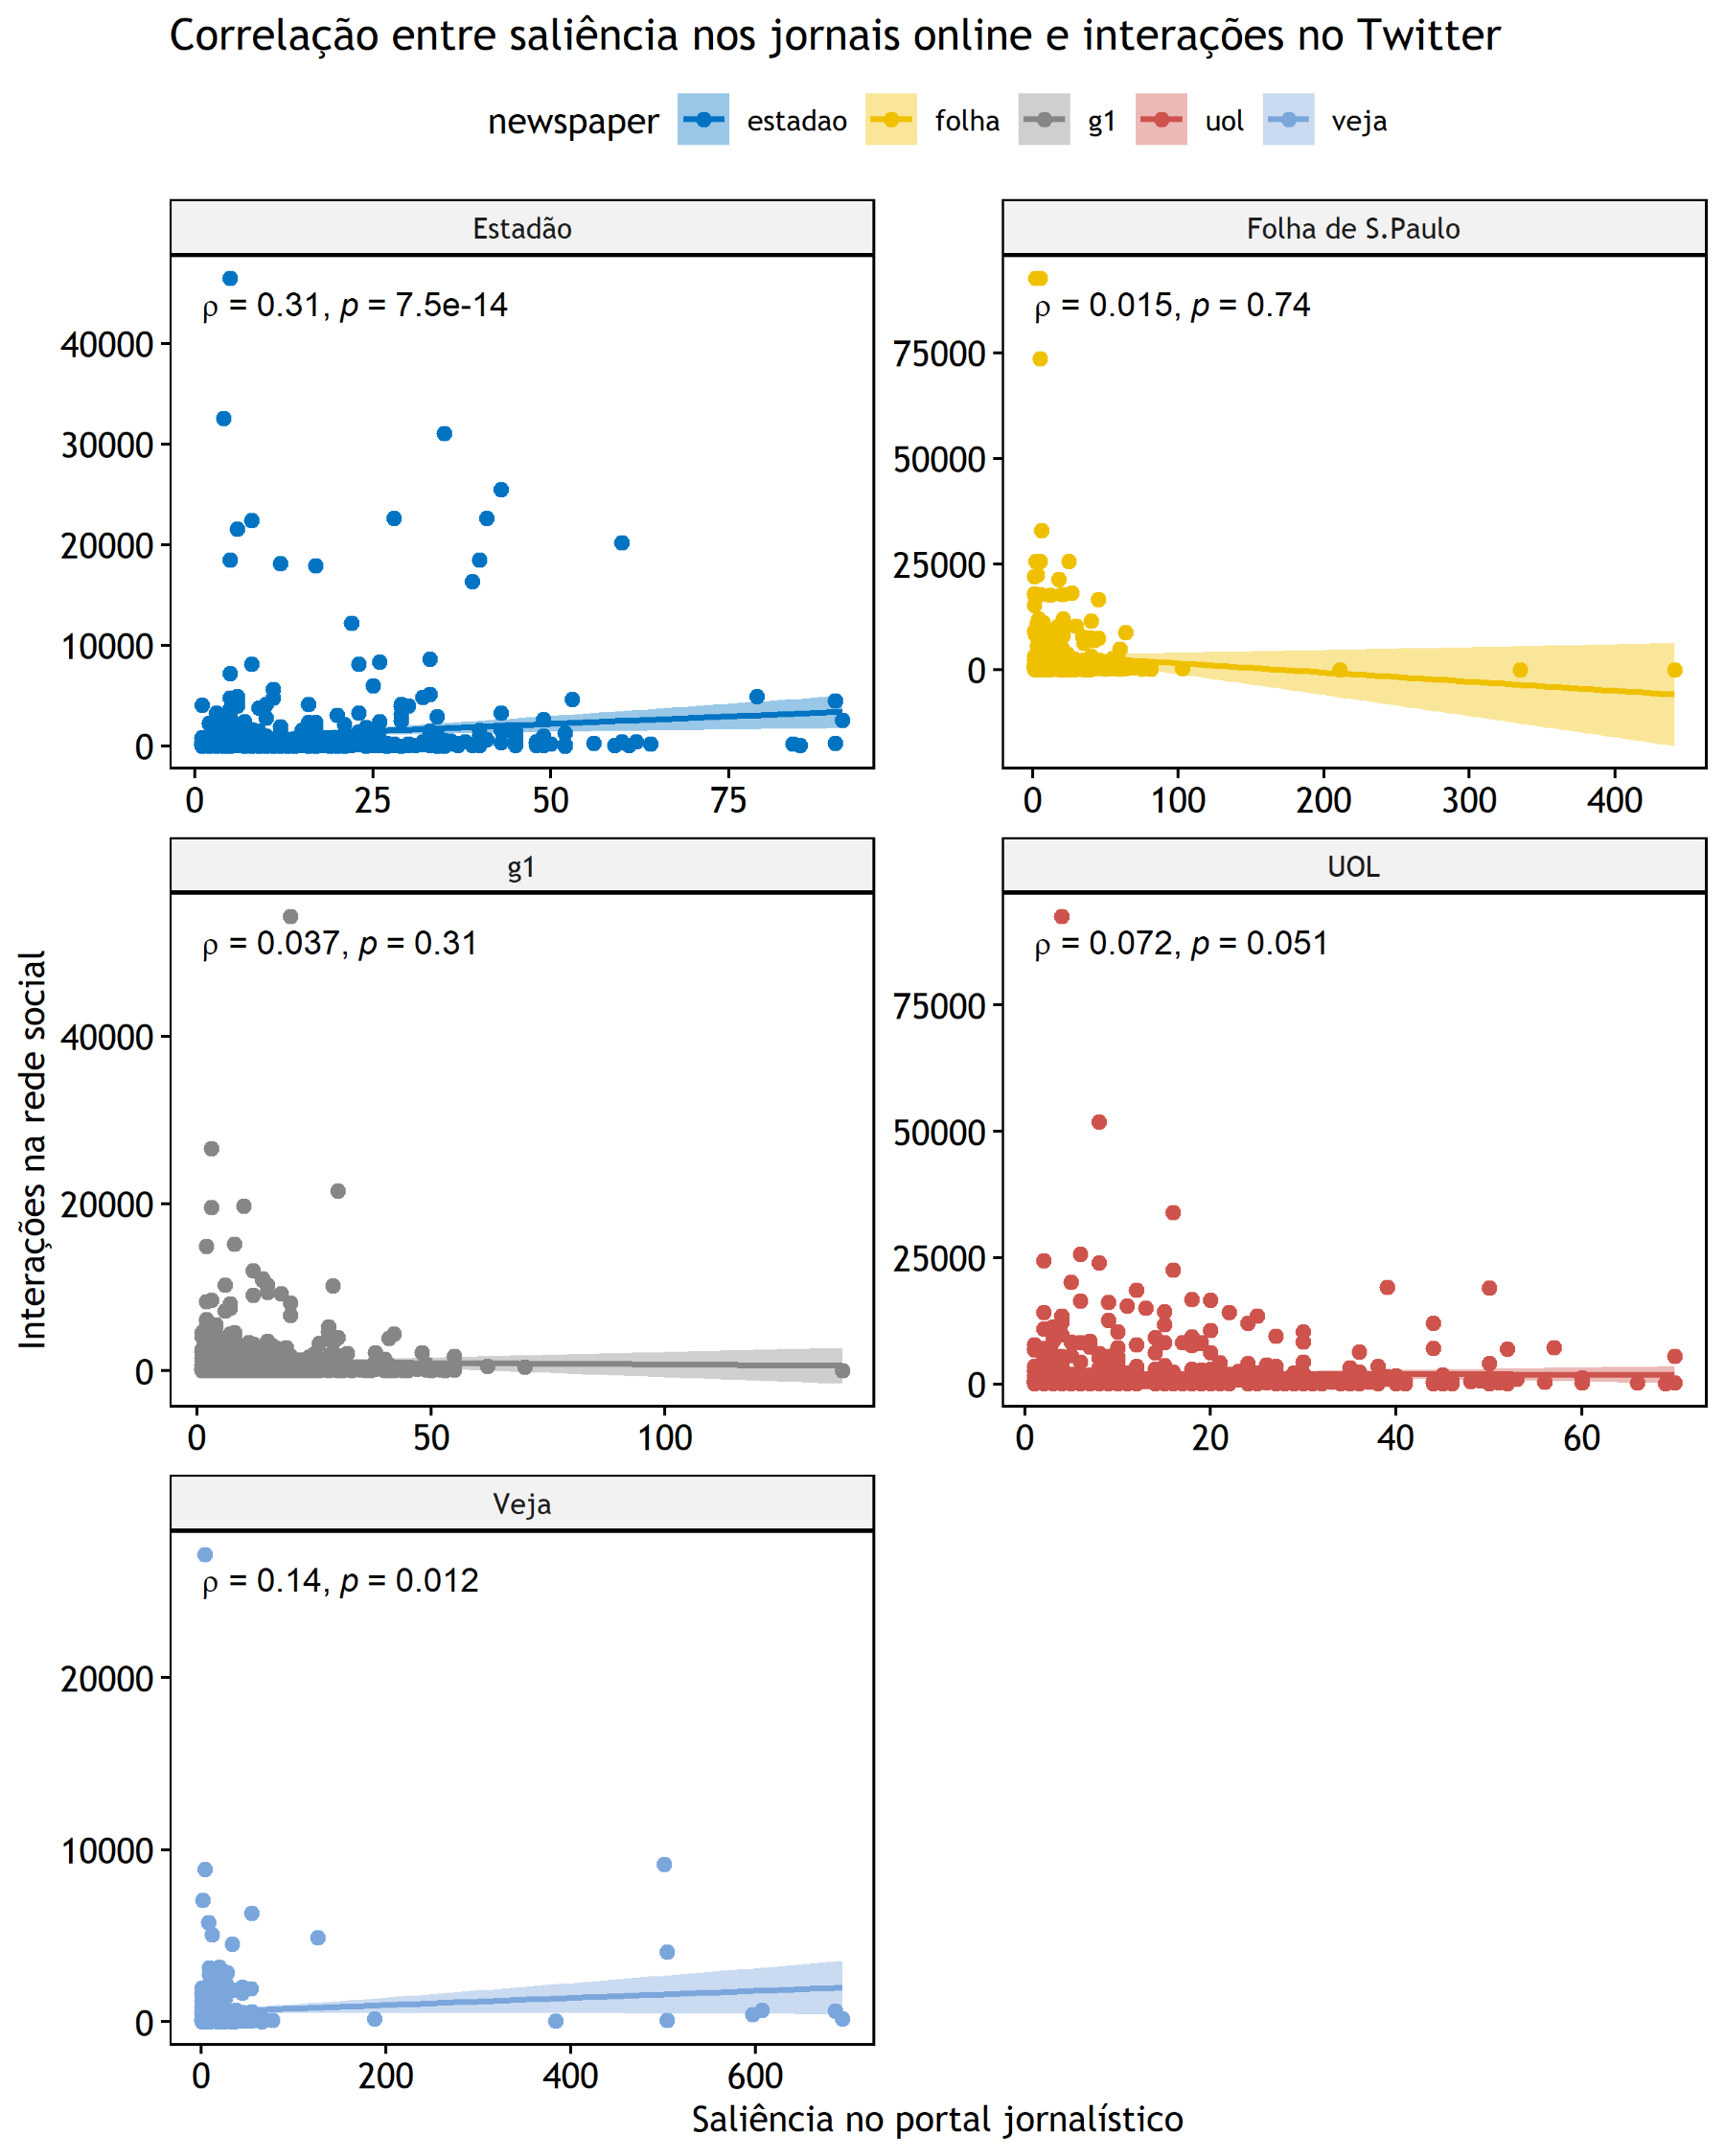
\includegraphics{twitter.png}
	\label{fig:correlacao-twitter}
  \source{Igor Antun, 2023}
\end{figure}

\begin{table}[H]
	\centering
	\caption{Correlação de Spearman - Twitter}
		\begin{tabular}{p{2in} p{1in} p{1in} p{1in} } \hline

		Jornal & $\rho$ & p-valor \\ \hline
		Estadão	& 0,31 & 7,5e-14 \\ 
		Folha de S.Paulo & 0,015 & 0,74 \\ 
		g1	& 0,037 & 0,31 \\ 
		UOL	& 0,072 & 0,051 \\ 
		Veja & 0,14 & 0,012 \\ \hline
		
		\end{tabular}
	\label{tab:correlacao-twitter}
  \source{Igor Antun, 2023}
\end{table}

No caso do Twitter, novamente encontramos um cenário onde o Estadão se mostra exceção frente aos outros jornais. Seu coeficiente de 0,31 do Estadão aponta para a existência de uma correlação fraca a moderada. Ademais, o p-valor próximo a zero também corrobora essa hipótese, afastando a possibilidade de isso se dar ao acaso.

Cabe mencionar também o caso da Veja, onde mais uma vez se conferiu um coeficiente de 0,14 e, nesse caso, com p-valor que possibilita a interpretação da existência de uma correlação fraca.

Os outros jornais, por sua vez, não apresentaram qualquer correlação.


\chapter{Conclusão}
Os resultados gerais apontam para a inexistência de correlação entre as agendas social e midiática no contexto das eleições de 2022 no Brasil. Ou seja, dentro do período analisado não comprovou-se relação significativa entre a saliência dada pelos jornais digitais às matérias observadas e o número de interações que estas obtiveram no Facebook ou no Twitter.

\postextual
\bibliography{referencias}

\end{document}
